\section{Introduction}
\label{sec:intro}
\begin{figure}[th]
    \centering
    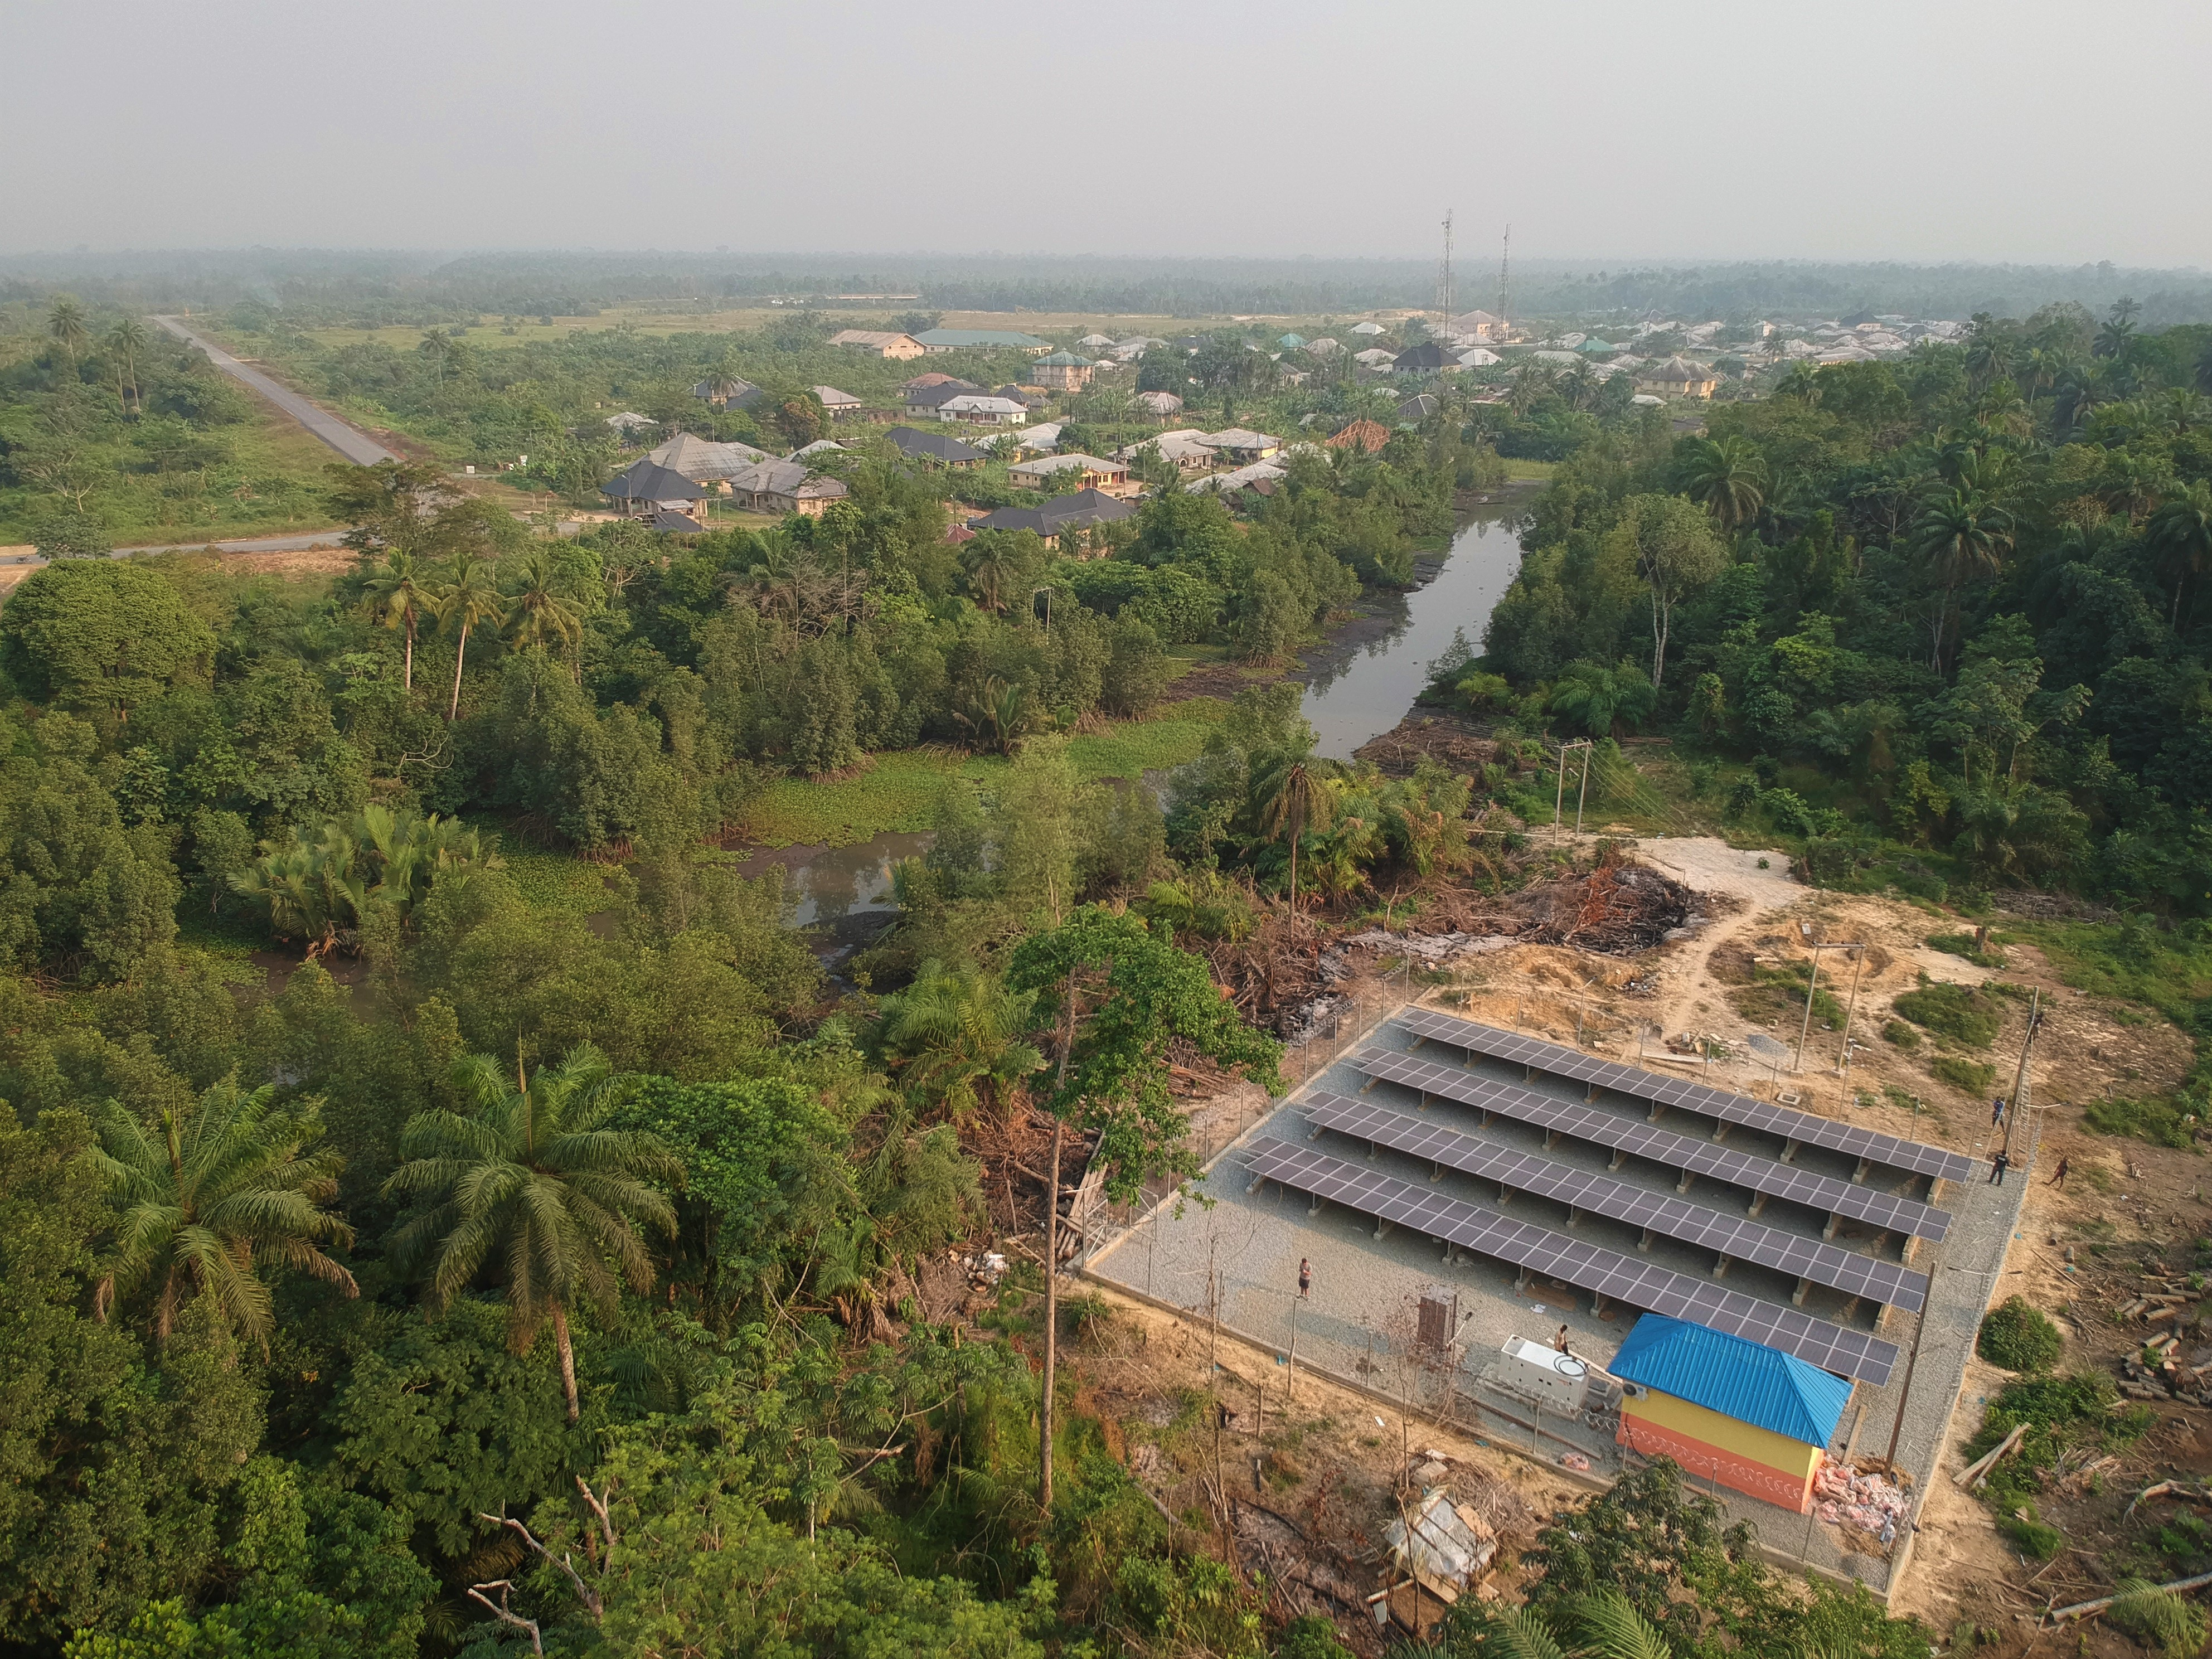
\includegraphics[width=0.8\textwidth]{images/mini-grid-bayelsa.jpg}
    \caption{A solar mini-grid in Bayelsa, Nigeria}
    \label{fig:mini-grid}
\end{figure}

Sub-Saharan Africa (SSA) has vast renewable energy resources, including solar, wind, hydropower, and geothermal \cite{hafner2018prospects}. However, these resources remain largely untapped, and the region is still heavily reliant on fossil fuels due to factors including a lack of infrastructure, financing, and technical expertise \cite{irena2022renewable}. Decentralized renewable energy solutions\textcolor{violet}{, especially renewable mini-grid (RMG) systems,} can offer a promising alternative to grid-based electricity in SSA \cite{moro2018ensuring, rasagam2018delivering}. RMG systems like the one illustrated in \cref{fig:mini-grid} are typically smaller in scale and can be installed in rural areas where grid extension is not feasible or cost-effective. RMG systems can also be operated by local communities, which can help to empower these communities and promote economic development \cite{deshmukh2009role, edwards2018role}.
Several studies have investigated the potential of RMGs as decentralized renewable energy solutions in SSA \cite{rabetanetiarimanana2018pv, okunlola2018assessment, moner2018electrification}. These studies have found that RMGs can have a significant positive impact on access to electricity, livelihoods, and economic development \cite{dawoud2018hybrid}. RMGs are small power grids that typically serve a few hundred to a few thousand households and businesses. They are often powered by renewable energy sources, such as solar or wind, and can provide a reliable and affordable source of electricity to communities that are not connected to the national grid.

Rural electrification is the process of providing fast, reliable, and affordable access to electricity to residents in rural areas who currently lack it. Access to electricity is seen as key to reducing poverty and is a critical component of economic development and poverty alleviation due to its ability to improve access to and quality of essential services such as education, healthcare, and clean water \cite{hussein2012analysis, hanjra2009reducing}. It can also create new employment opportunities and boost agricultural productivity. SSA has the lowest electrification rate in the world and the majority of those without access live in rural areas due to lack of financial ability to extend the grid, population density, and other social and cultural factors \cite{zebra2021review}. Data from a 2019 World Bank report shows that 14 of the 20 countries in the world with the highest deficit in electricity connections are African countries \cite{Tracking_SDG7_Report_2019}. Only $45\%$ of the population in SSA currently have access to electricity. The electrification coverage is expected to rise to only about $60\%$ of the SSA population by 2030 given current conditions \cite{valickova2021costs}. Despite representing approximately $14\%$ of the world's population, SSA accounts for only about $4\%$ of global energy consumption \cite{falk2021socio}.

Rural electrification can significantly benefit communities \cite{chakravorty2016lighting}. According to \cite{falk2021socio}, the introduction of electrification via RMG has had significant positive impacts on socioeconomic factors such as health care and economic development. RMG systems promote faster and more flexible energy supply, especially when integrated with additional components such as electricity storage in a hybrid system \cite{mazzeo2021literature}. The slow extension of conventional grid systems has led to increased interest in RMGs, a decentralized alternative not connected to the public grid and generating electricity based on various technologies \cite{korkovelos2020retrospective}. According to \cite{valickova2021costs}, the incremental cost of providing electricity access to households is below the cost of alternatives such as kerosene lighting.

Various socioeconomic factors affect rural electrification in SSA. According to \cite{poblete2021model}, income levels are a key driver of rural electrification. As incomes rise, households are more likely to be able to afford more electricity and appliances. The rising demand in RMGs due to growing populations, industrial growth, and government policies can play a significant role in promoting rural electrification \cite{antonanzas2021state}. Technological advancements also play an important role in rendering the electrification process more feasible and affordable to provide electricity to rural areas. Moreover, digital and information technologies have several positive effects on the development and regulation of efficient energy consumption \cite{shabalov2021influence, Consultant_Klooss_Consultant_2021}.

While existing research has acknowledged the significance of social impacts stemming from RMG implementation in SSA, there remains a notable absence in empirical measurements \cite{eales2018social}. The prevailing studies predominantly focus on technical and economic aspects, neglecting the quantification of social ramifications \cite{pueyo2018impact, wassie2021socio, uwineza2021analysis, lee2020experimental}. A recent study in the Gbamu Gbamu village in Nigeria uses a combination of statistical tests to measure the financial impact of RMGs on local businesses using predominantly economic factors including gender, marital status, household size, age, education level, years of business establishment, hours of operation, building tenure, capital source, number of employees, generator ownership, and the days of operation \cite{babalola2022socio}. 

A few studies have attempted to formally quantify social impacts of RMGs on communities. In \cite{liu2021enabling}, researchers apply a mediation model to illustrate how community engagement results in a  $1\%$ increase in the perceived renewable energy potential, leading to a $0.195\%$ increase in perceived poverty reduction. These results suggest that community empowerment is indispensable in creating electricity demand and delivering development impact of renewable RMGs in the context of deep poverty. In another study carried out in Kyenjojo District in western Uganda, the authors incorporated social factors in a study of RMG  operation, causes of failure, sources of discomfort to customers, and customer behavior \cite{cartland2022socio}. Moreover, researchers in \cite{duran2021analysis} conducted a systematic review of diverse RMG projects aimed at extracting qualitative insights into the factors driving project success and community benefits. Subsequently, these findings were empirically validated, enabling the identification of key factors contributing to the success and cost-effectiveness of RMG projects \cite{nyarko2023drivers}. These studies have highlighted the necessity for broader assessments that go beyond solely examining economic impacts and RMG operational challenges in rural areas relying on RMGs. We aim to broaden this perspective by considering both economic and social factors like gender equality and community residents' safety. This shift recognizes the interconnection between socioeconomic elements, addressing a significant gap in understanding the overall transformational impact of RMG initiatives within rural settings. 

Our study aims to bridge the gap in empirical measurement of social impact of RMGs on rural communities by introducing a comprehensive framework that delineates five crucial axes encompassing gender equality, productivity, health, safety, and economic activity. By leveraging a survey designed specifically around these axes, we endeavor to quantify the multifaceted impacts of solar RMGs on various social and economic factors within rural African communities. Unlike previous single-region analyses, our research embraces a comparative approach, drawing insights from two distinct countries, Kenya and Nigeria. This deliberate expansion of our dataset \textcolor{violet}{yields} a richer understanding of the nuanced effects of RMG interventions across diverse sociocultural landscapes. The rest of the paper is organized as follows. In \cref{sec:methodology}, we discuss the model, data, and estimation techniques. The results and findings are presented in \cref{sec:results}. Further discussion and methodology limitations are shown in \cref{sec:discussion}. We conclude in \cref{sec:conclusion}.